% Source: Code/ML_overlay/ir_rgb_registration/paper/figures/fig_data_pipeline.tex
% Data Pipeline and Ground Truth Generation
% IR/RGB Registration — Journal Figure
\documentclass[tikz,border=4pt]{standalone}

\usepackage[T1]{fontenc}
\usepackage{lmodern}
\usepackage{amsmath}
\usepackage{amssymb}

\usetikzlibrary{arrows.meta, positioning, calc, fit, decorations.pathreplacing}

% --- Brand Colors ---
\definecolor{Garnet}{HTML}{73000A}
\definecolor{Atlantic}{HTML}{466A9F}
\definecolor{Congaree}{HTML}{1F414D}
\definecolor{Horseshoe}{HTML}{65780B}
\definecolor{WarmGrey}{HTML}{676156}
\definecolor{Sandstorm}{HTML}{FFF2E3}
\definecolor{Black90}{HTML}{363636}
\definecolor{Black70}{HTML}{5C5C5C}
\definecolor{Black50}{HTML}{A2A2A2}
\definecolor{Black30}{HTML}{C7C7C7}
\definecolor{Black10}{HTML}{ECECEC}
\definecolor{Rose}{HTML}{CC2E40}

\begin{document}
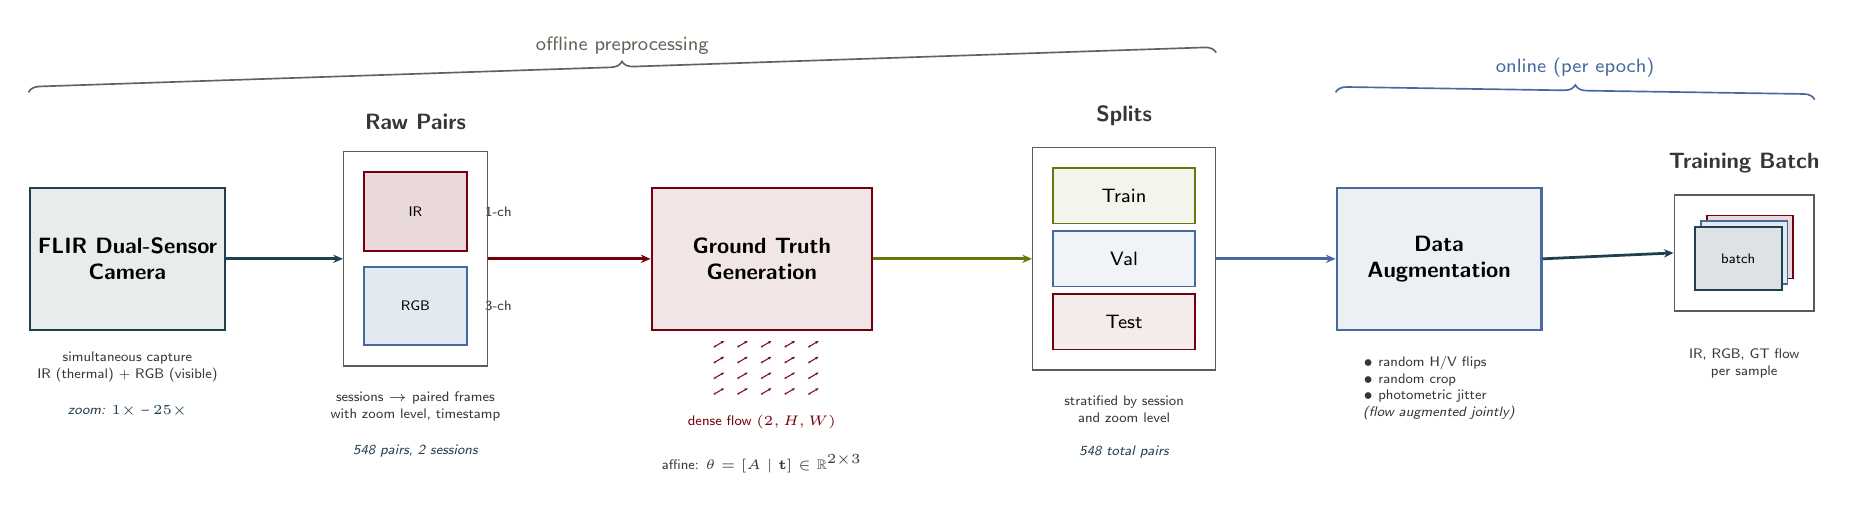
\begin{tikzpicture}[
    >=Stealth,
    font=\sffamily\small,
    % --- Pipeline stage block ---
    stage/.style={
        draw=#1, fill=#1!10, line width=0.8pt,
        minimum height=14mm, minimum width=22mm,
        inner sep=3pt, align=center,
        font=\sffamily\footnotesize\bfseries,
    },
    % --- Small data card ---
    datacard/.style={
        draw=#1, fill=#1!8, line width=0.6pt,
        minimum height=7mm, minimum width=14mm,
        inner sep=2pt, align=center,
        font=\sffamily\scriptsize,
    },
    % --- Image thumbnail placeholder ---
    imgbox/.style={
        draw=#1, fill=#1!15, line width=0.7pt,
        minimum height=10mm, minimum width=13mm,
        inner sep=0pt, align=center,
        font=\sffamily\tiny,
    },
    % --- Dimension / annotation label ---
    dimlab/.style={
        font=\sffamily\tiny, text=Black90,
    },
    % --- Arrow styles ---
    thickarrow/.style={
        -{Stealth[length=3.5pt,width=3pt]},
        line width=1.0pt, color=#1,
    },
    % --- Brace decoration (opens upward) ---
    pipebrace/.style={
        decorate, decoration={brace, amplitude=4pt},
        line width=0.6pt, draw=#1,
    },
]

% =====================================================================
% STAGE 1: FLIR DUAL-SENSOR CAMERA
% =====================================================================
\node[stage=Congaree, minimum width=24mm, minimum height=18mm] (camera) at (0,0)
    {FLIR Dual-Sensor\\Camera};

% Camera details below
\node[dimlab, below=1.5mm of camera, align=center] (cam_info)
    {simultaneous capture\\IR (thermal) + RGB (visible)};

% Zoom range annotation
\node[dimlab, below=0.5mm of cam_info, text=Congaree, font=\sffamily\tiny\itshape] (zoom_info)
    {zoom: $1\times$ -- $25\times$};

% =====================================================================
% STAGE 2: RAW PAIRED DATA
% =====================================================================
\coordinate (raw_center) at ($(camera.east) + (24mm, 0)$);

% IR thumbnail
\node[imgbox=Garnet] (ir_thumb) at ($(raw_center) + (0, 6mm)$) {IR};
\node[dimlab, right=1mm of ir_thumb] {1-ch};

% RGB thumbnail
\node[imgbox=Atlantic] (rgb_thumb) at ($(raw_center) + (0, -6mm)$) {RGB};
\node[dimlab, right=1mm of rgb_thumb] {3-ch};

% Bounding box around pair
\node[draw=Black70, line width=0.5pt, inner sep=2.5mm,
      fit=(ir_thumb)(rgb_thumb)] (raw_box) {};

% Label above the box
\node[font=\sffamily\footnotesize\bfseries, text=Black90,
      above=1.5mm of raw_box] (raw_label) {Raw Pairs};

% Metadata annotation
\node[dimlab, below=2mm of raw_box, align=center] (raw_meta)
    {sessions $\rightarrow$ paired frames\\with zoom level, timestamp};

% Dataset stats
\node[dimlab, below=0.5mm of raw_meta, text=Congaree, font=\sffamily\tiny\itshape]
    (stats_raw) {548 pairs, 2 sessions};

% =====================================================================
% STAGE 3: GROUND TRUTH GENERATION
% =====================================================================
\coordinate (gt_center) at ($(raw_center) + (44mm, 0)$);

\node[stage=Garnet, minimum width=28mm, minimum height=18mm] (gt_block)
    at (gt_center) {Ground Truth\\Generation};

% Flow field visual: grid with displacement arrows below the block
\begin{scope}[shift={($(gt_block.south) + (0, -5mm)$)}]
    \foreach \x in {-6mm, -3mm, 0mm, 3mm, 6mm} {
        \foreach \y in {-3mm, -1mm, 1mm, 3mm} {
            \fill[Garnet!60] (\x, \y) circle (0.5pt);
            \draw[Garnet, line width=0.35pt, -{Stealth[length=1.2pt,width=1pt]}]
                (\x, \y) -- ++(1.2mm, 0.7mm);
        }
    }
    \node[dimlab, below=1.5mm, text=Garnet, anchor=north] at (0, -3mm)
        {dense flow $(2,H,W)$};
\end{scope}

% GT details below the flow field
\node[dimlab, below=14.5mm of gt_block, align=center] (gt_details) {%
    affine: $\theta = [A \mid \mathbf{t}] \in \mathbb{R}^{2\times 3}$};

% =====================================================================
% STAGE 4: TRAIN / VAL / TEST SPLITS
% =====================================================================
\coordinate (split_center) at ($(gt_center) + (46mm, 0)$);

% Three split boxes stacked
\node[datacard=Horseshoe, minimum width=18mm] (split_train)
    at ($(split_center) + (0, 8mm)$) {Train};
\node[datacard=Atlantic, minimum width=18mm] (split_val)
    at ($(split_center) + (0, 0mm)$) {Val};
\node[datacard=Garnet, minimum width=18mm] (split_test)
    at ($(split_center) + (0, -8mm)$) {Test};

% Bounding box
\node[draw=Black70, line width=0.5pt, inner sep=2.5mm,
      fit=(split_train)(split_test)] (split_box) {};

% Label above the box
\node[font=\sffamily\footnotesize\bfseries, text=Black90,
      above=1.5mm of split_box] (split_label) {Splits};

% Split info
\node[dimlab, below=2mm of split_box, align=center] (split_info)
    {stratified by session\\and zoom level};

\node[dimlab, below=0.5mm of split_info, text=Congaree, font=\sffamily\tiny\itshape]
    {548 total pairs};

% =====================================================================
% STAGE 5: DATA AUGMENTATION
% =====================================================================
\coordinate (aug_center) at ($(split_center) + (40mm, 0)$);

\node[stage=Atlantic, minimum width=26mm, minimum height=18mm] (aug_block)
    at (aug_center) {Data\\Augmentation};

% Augmentation list
\node[dimlab, below=2mm of aug_block, align=left, anchor=north] (aug_list) {%
    {\tiny$\bullet$} random H/V flips\\
    {\tiny$\bullet$} random crop\\
    {\tiny$\bullet$} photometric jitter\\
    {\tiny\textit{(flow augmented jointly)}}};

% =====================================================================
% STAGE 6: TRAINING BATCH
% =====================================================================
\coordinate (batch_center) at ($(aug_center) + (38mm, 0)$);

% Stacked batch representation
\node[imgbox=Garnet, minimum width=11mm, minimum height=8mm]
    (batch3) at ($(batch_center) + (1.5mm, 1.5mm)$) {};
\node[imgbox=Atlantic, minimum width=11mm, minimum height=8mm]
    (batch2) at ($(batch_center) + (0.75mm, 0.75mm)$) {};
\node[imgbox=Congaree, minimum width=11mm, minimum height=8mm,
      fill=Congaree!15, font=\sffamily\tiny]
    (batch1) at (batch_center) {batch};

% Bounding box
\node[draw=Black70, line width=0.5pt, inner sep=2.5mm,
      fit=(batch1)(batch3)] (batch_box) {};

% Label above the box
\node[font=\sffamily\footnotesize\bfseries, text=Black90, align=center,
      above=1.5mm of batch_box] (batch_label) {Training Batch};

% Batch info
\node[dimlab, below=3.5mm of batch_box, align=center] (batch_info)
    {IR, RGB, GT flow\\per sample};

% =====================================================================
% ARROWS: Main pipeline flow (left to right)
% =====================================================================
\draw[thickarrow=Congaree] (camera.east) -- (raw_box.west);
\draw[thickarrow=Garnet]   (raw_box.east) -- (gt_block.west);
\draw[thickarrow=Horseshoe](gt_block.east) -- (split_box.west);
\draw[thickarrow=Atlantic] (split_box.east) -- (aug_block.west);
\draw[thickarrow=Congaree] (aug_block.east) -- (batch_box.west);

% =====================================================================
% TOP BRACES: Offline preprocessing vs. Online training
% Placed above the labels with enough clearance
% =====================================================================
% Compute a uniform top-line above all stage labels
\coordinate (brace_y_offline) at ($(raw_label.north) + (0, 3mm)$);
\coordinate (brace_y_online)  at ($(batch_label.north) + (0, 3mm)$);

% Offline brace: camera to splits
\draw[pipebrace=WarmGrey]
    ($(camera.north west) + (0, 12mm)$) --
    ($(split_box.north east) + (0, 12mm)$)
    node[midway, above=3pt, font=\sffamily\scriptsize, text=WarmGrey]
    {offline preprocessing};

% Online brace: augmentation to training batch
\draw[pipebrace=Atlantic]
    ($(aug_block.north west) + (0, 12mm)$) --
    ($(batch_box.north east) + (0, 12mm)$)
    node[midway, above=3pt, font=\sffamily\scriptsize, text=Atlantic]
    {online (per epoch)};

\end{tikzpicture}
\end{document}
